\subsection{Baseline}

\textbf{Motivation.} Experiments that will follow will focus on trying out different feature sets, so it is natural to keep every other variable constant. Since the dataset is fixed and the feature set is going to be changing, it remains to find acceptable values for the network architecture and the training hyperparameters. 

Due time and resources constraints, I decided to set the training hyperparameters to   (similar) values which give good results in the official Stockfish trainer: \textbf{a batch size of 16384, a learning rate of 0.0005 and a exponential decay factor of 0.99}. This values showed acceptable results during early stages of development and will remain fixed for all runs.

It remains to find a good network architecture. Bigger networks may have lower loss and predict better, but they will also have slower inferences. This is the tradeoff between inference time and node visits (more depth), which are also affected by the quality of the prediction due to better pruning. So the model must be so much better to compensate the slowdown in inference. \\

\textbf{Experiment.}  In this first experiment I will try different sizes of L1 and L2,  to find an acceptable tradeoff for future experiments. I will run a grid search with L1 $\in \{256, 512, 1024, 2048\}$ and L2 $\in \{32, 64, 128, 256\}$. The feature set used to train will be \featureset{All}, the canonical set with 768 features.

I expect that there will be a model that performs best and other models that are smaller (need stronger predictions) and bigger (need speed to visit more nodes) perform worse. \\

\textbf{Results.} Looking at the result heatmaps in Figure \ref{fig:baseline_heatmaps}, the first thing to notice is that training and validation losses behave as expected. If the model is more complex, meaning the number of parameters (which is dominated by $768*L1+L1*L2$) is higher, the loss is lower and the model predicts better.

When the models are loaded into the engine and evaluated in a tournament, we can see that when L2 drops, the performance drops dramatically. This is due the fact that the inference time is mostly dominated by L2. This result suggests that it may be a good idea explore even lower values of L2, such as 16 or even 8. However, the SIMD implementation requires L2 to be a multiple of 32 so it needs a refactor to keep being fast. So, instead of fiddling further with SIMD I decided to \textbf{keep L2 at 32}.

\begin{figure}[H]
\centering
\makebox[\textwidth]{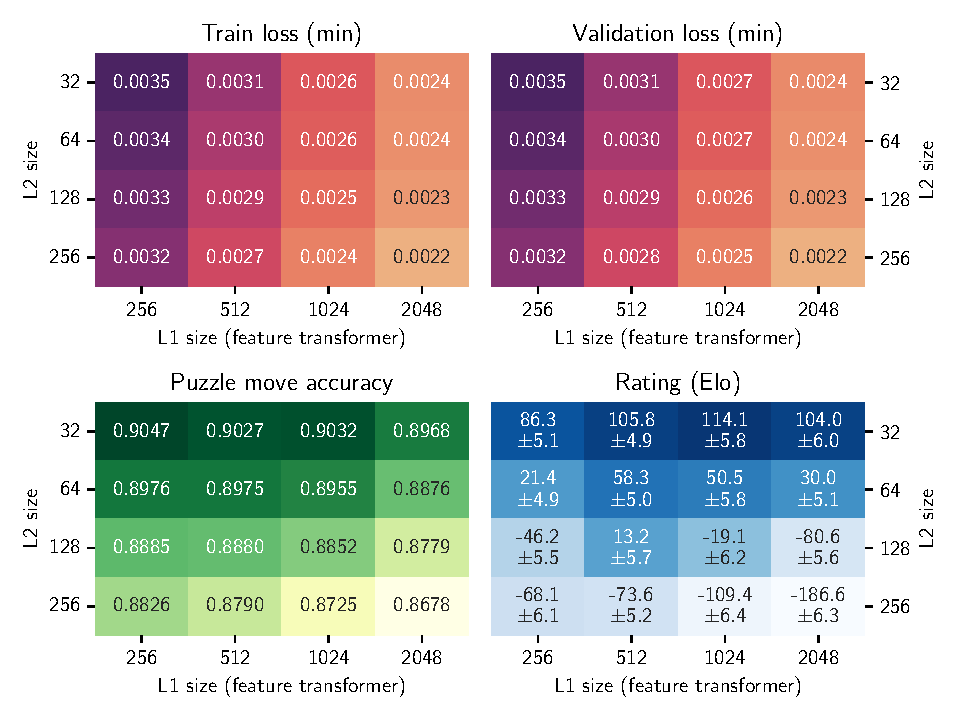
\includegraphics[width=\textwidth]{./dynamic/output/baseline_heatmaps.pdf}}
\captionsetup{justification=centering}
\caption{Network architecture sweep results (L1 $\times$ L2).\\ Table with details in Appendix \ref{appendix:baseline}.}
\label{fig:baseline_heatmaps}
\end{figure}

If L2 is kept constant, the best L1 is not the smallest nor biggest. If L2 $=64$ or L2 $=128$ there is a clear lead of L1 $=512$ in both. In the case of L2 $=32$, the best L1 is not clear because the differences in rating are small and are within margin of error, excluding L1 $=256$ which is definitely wrose. Because training lower values of L1 is faster I opted for \textbf{L1} $\bm{=512}$ due the difference being small and being the best in other L2 values.

So, further experiments will use L1 $=512$ and L2 $=32$. For reference, Stockfish currently uses L1=2560, and employ (lots of) more tricks to make it even faster. The values selected here are specific to the current implementation of the engine, since it may change if more optimizations are made (tradeoff is altered). For this reason, no further modifications to the engine were made after starting with the experiments. We can now proceed with more interesting experiments.
